\appendix

\chapter{Simulation Results}

Here are listed additional plots generated from the simulations. The plots show the percentage change of isotopes in the simulation with different thorium concentrations. 

\begin{figure}[h]
    \centering
    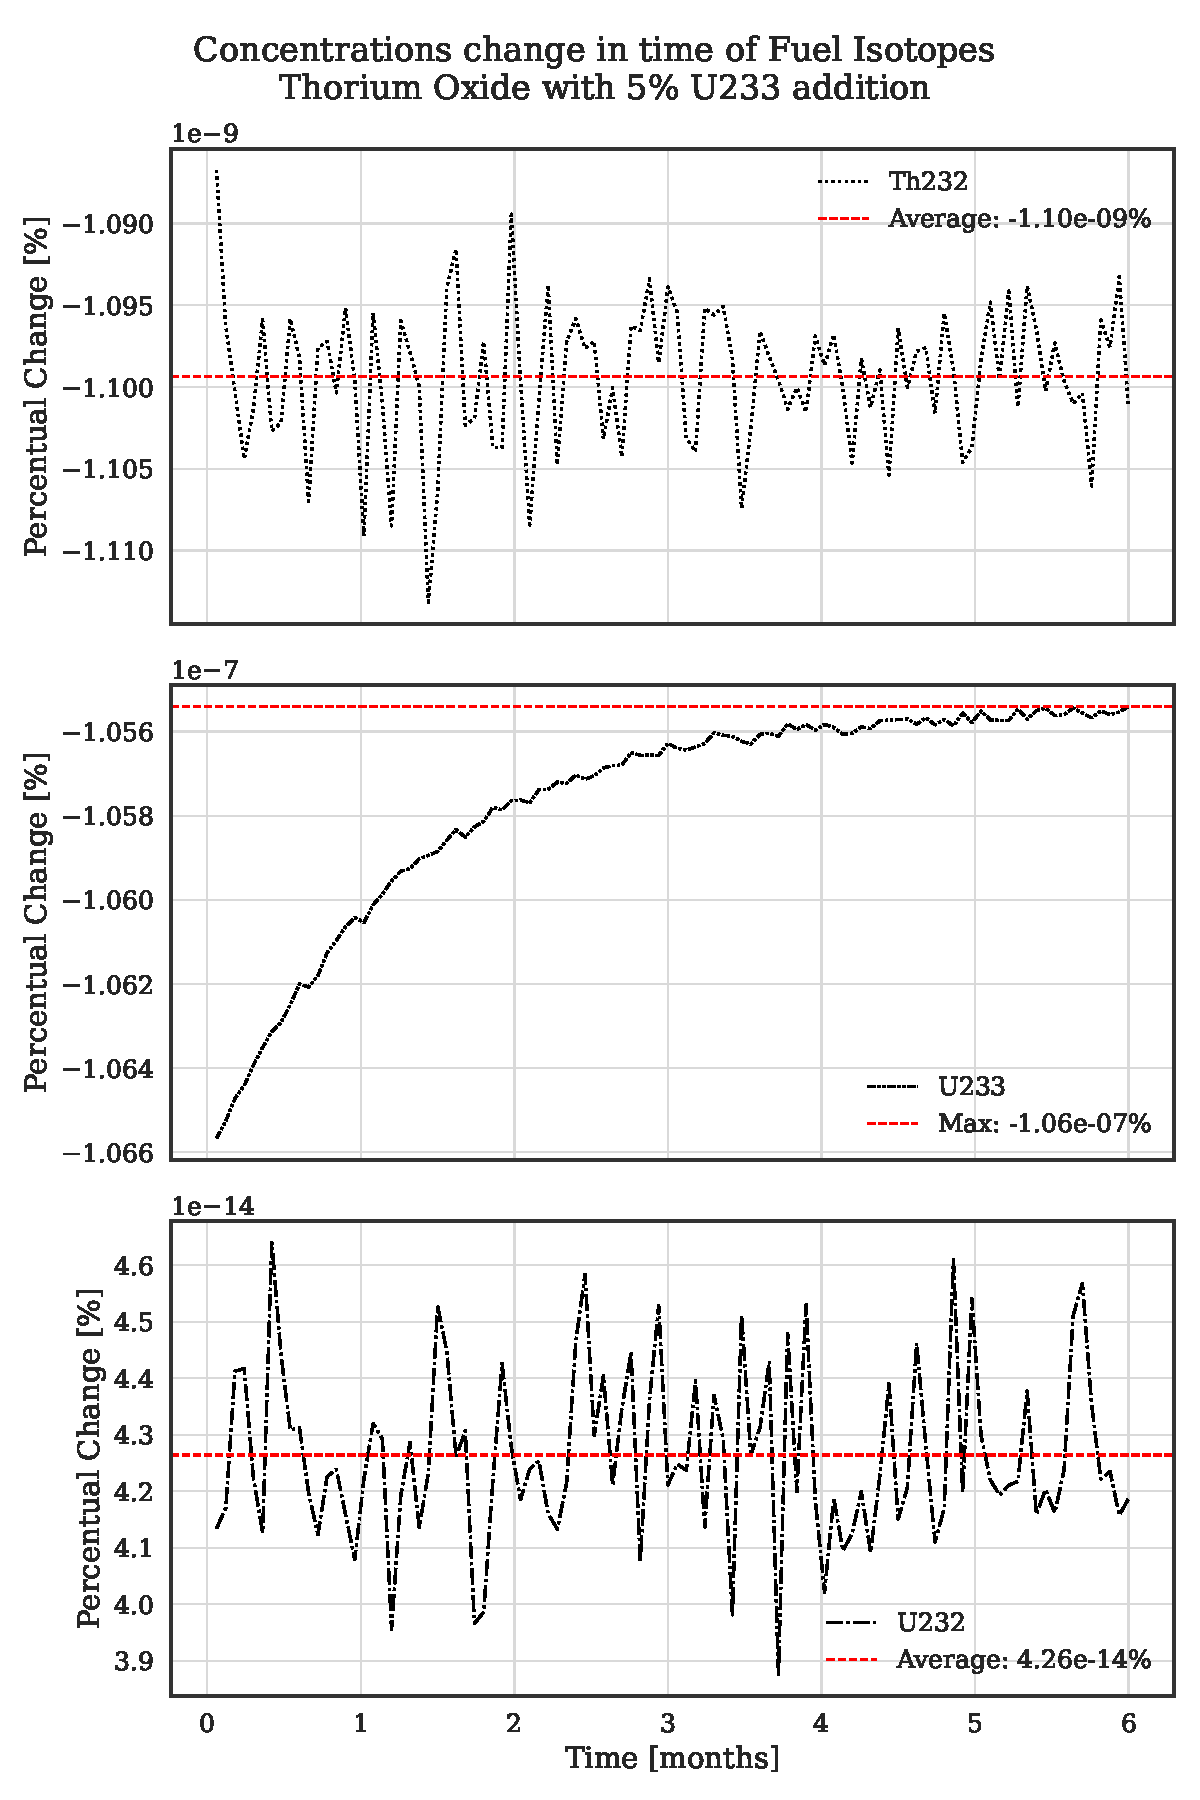
\includegraphics[width=0.75\textwidth, height=0.75\textheight]{Kap7/Figures_Kap7/percentual_change_th232_U233_5.pdf}
    \caption{Percentage change of isotopes in the simulation of a PWR fuel assembly using ThOX at \(5 \, \%\) \(\prescript{233}{}{U}\) concentration.}
    \label{fig:th_u233_5}
\end{figure}

\begin{figure}[h]
    \centering
    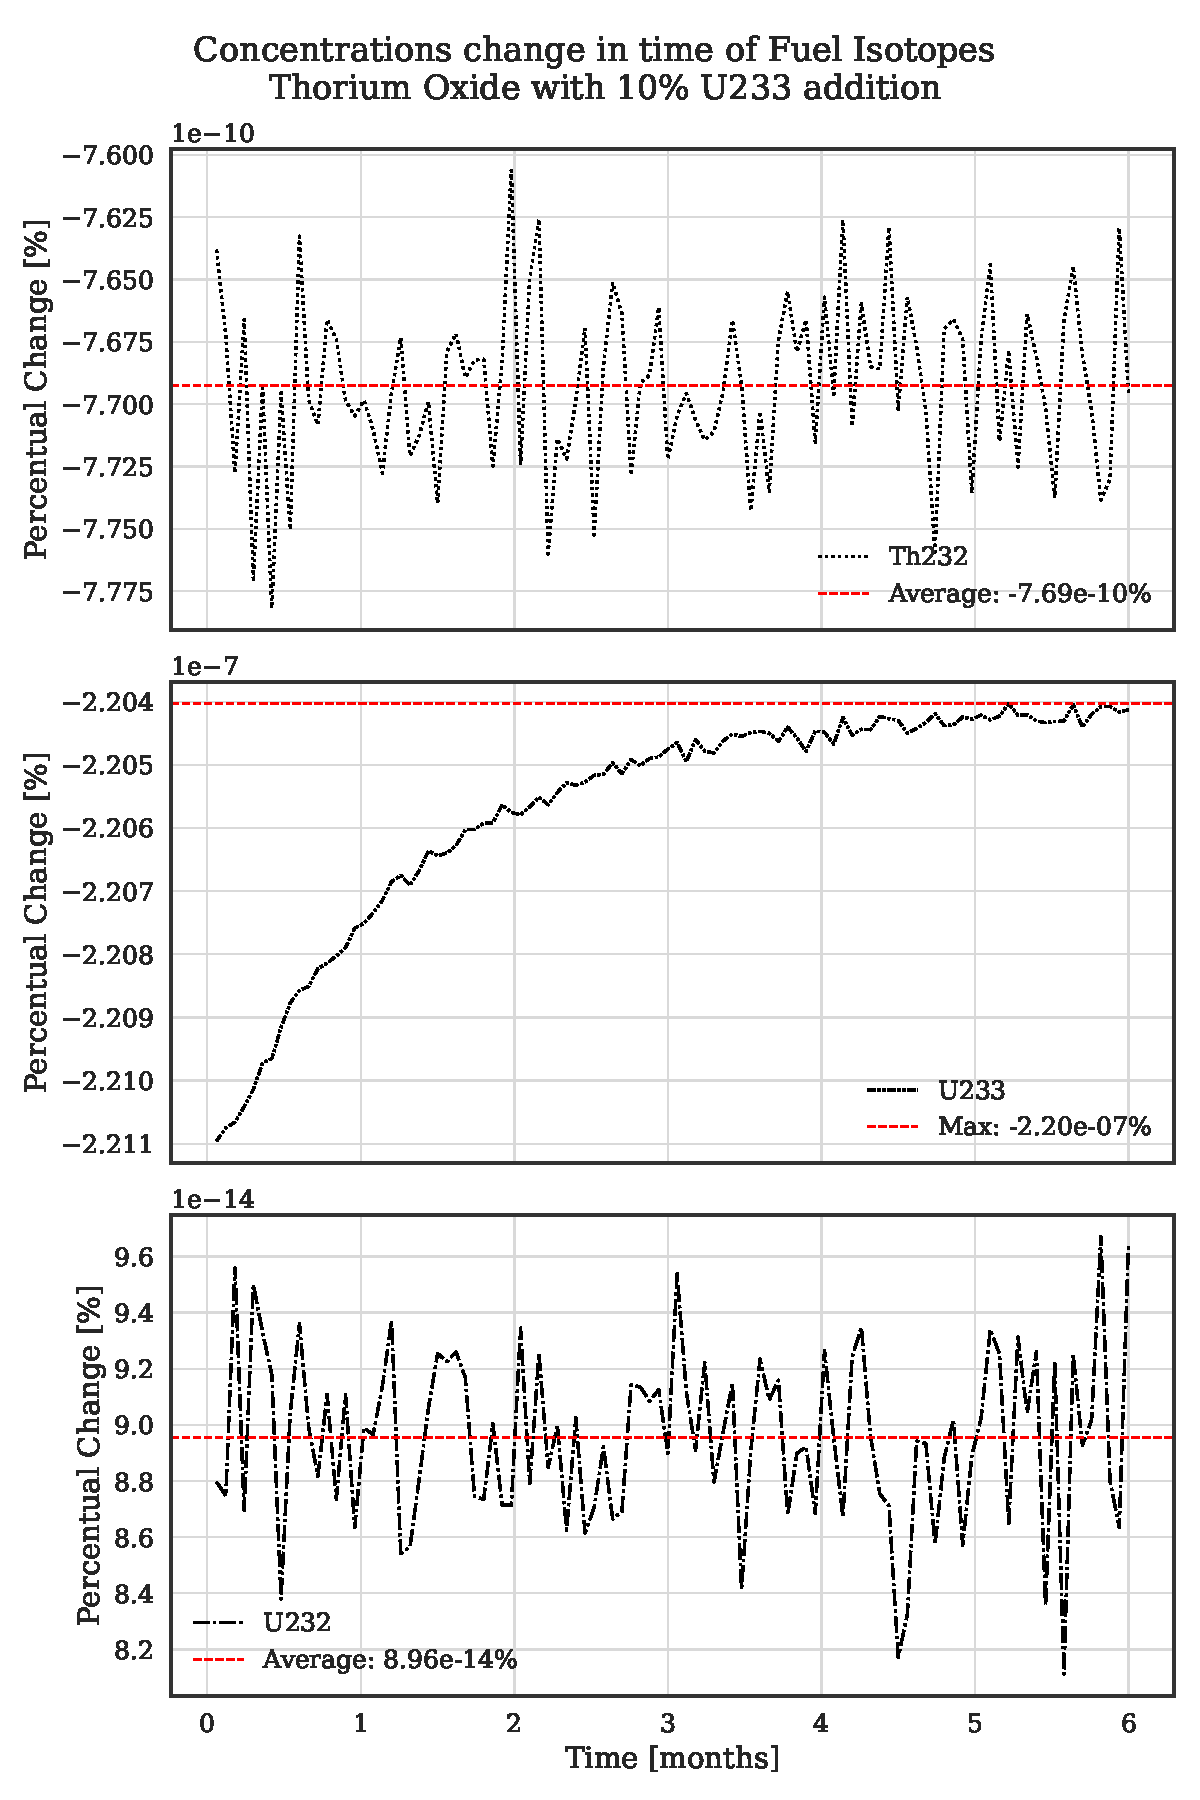
\includegraphics[width=0.75\textwidth, height=0.75\textheight]{Kap7/Figures_Kap7/percentual_change_th232_U233_10.pdf}
    \caption{Percentage change of isotopes in the simulation of a PWR fuel assembly using ThOX at \(10 \, \%\) \(\prescript{233}{}{U}\) concentration.}
    \label{fig:th_u233_10}
\end{figure}


 Reactivity behavior of the fuel assemblies during the simulation. The reactivity is calculated as in \textbf{Eq} (\ref{eq:def_reactivity}). It is noticeable that the reactivity of UOX, used as reference, is higher than \(0\). This is because the simulation is run from the beginning of the cycle, where it is needed this reactivity excess to ensure criticality of the reactor through the whole cycle.

\begin{figure}
    \centering
    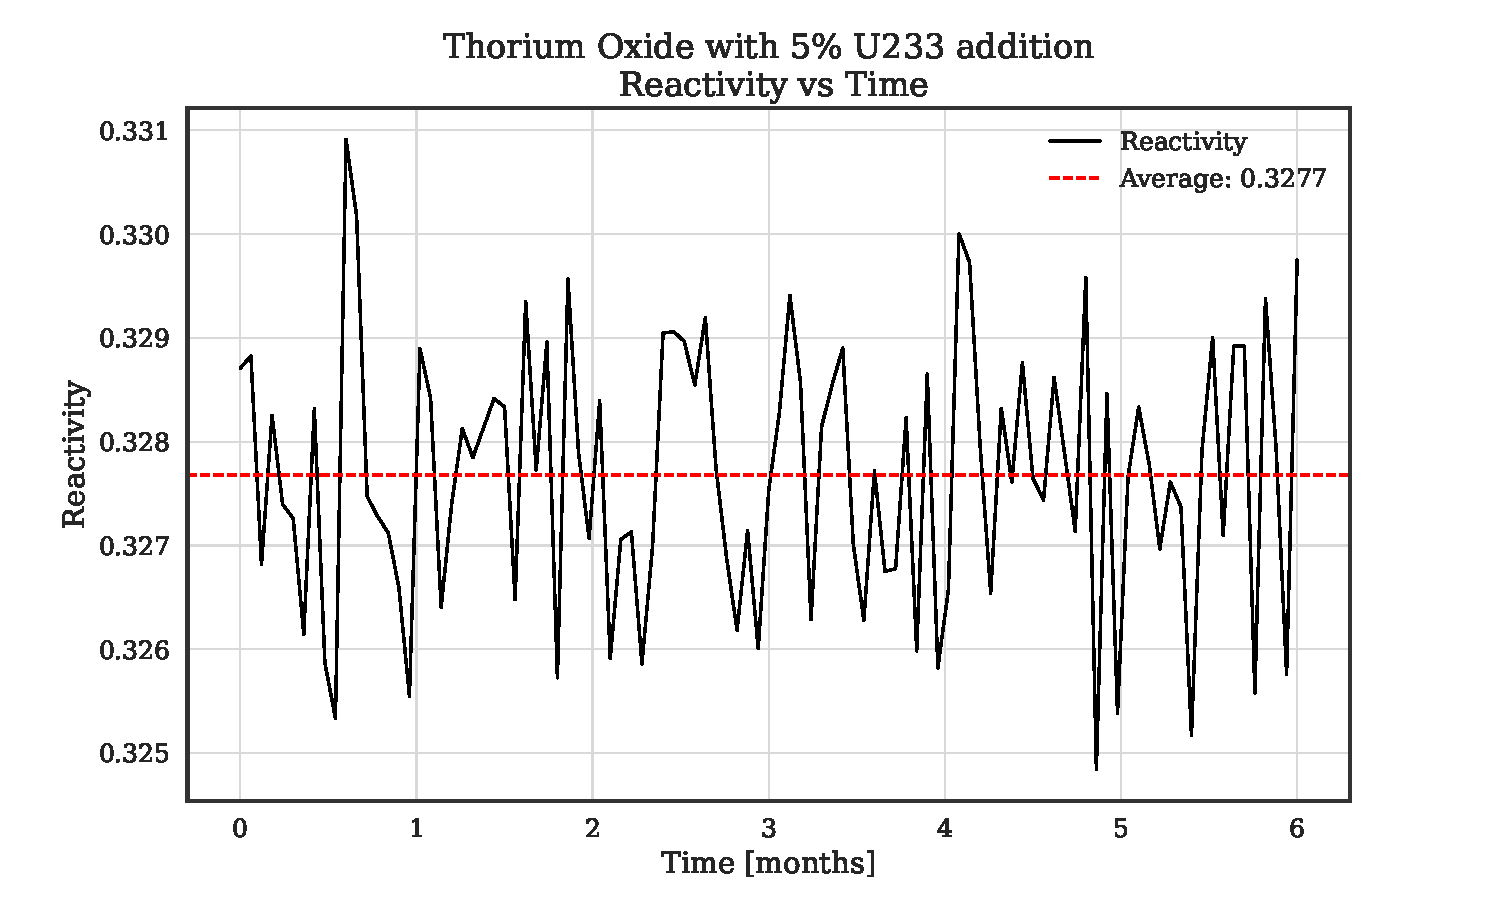
\includegraphics[width=0.75\textwidth, scale=0.75]{Kap7/Figures_Kap7/Reactivity_vs_Time_ThOX_U233_5.pdf}
    \caption{Reactivity of the simulation of a PWR fuel assembly using ThOX at \(5 \, \%\) \(\prescript{233}{}{U}\) concentration.}
    \label{fig:reactivity_th_u233_5}
\end{figure}

\begin{figure}
    \centering
    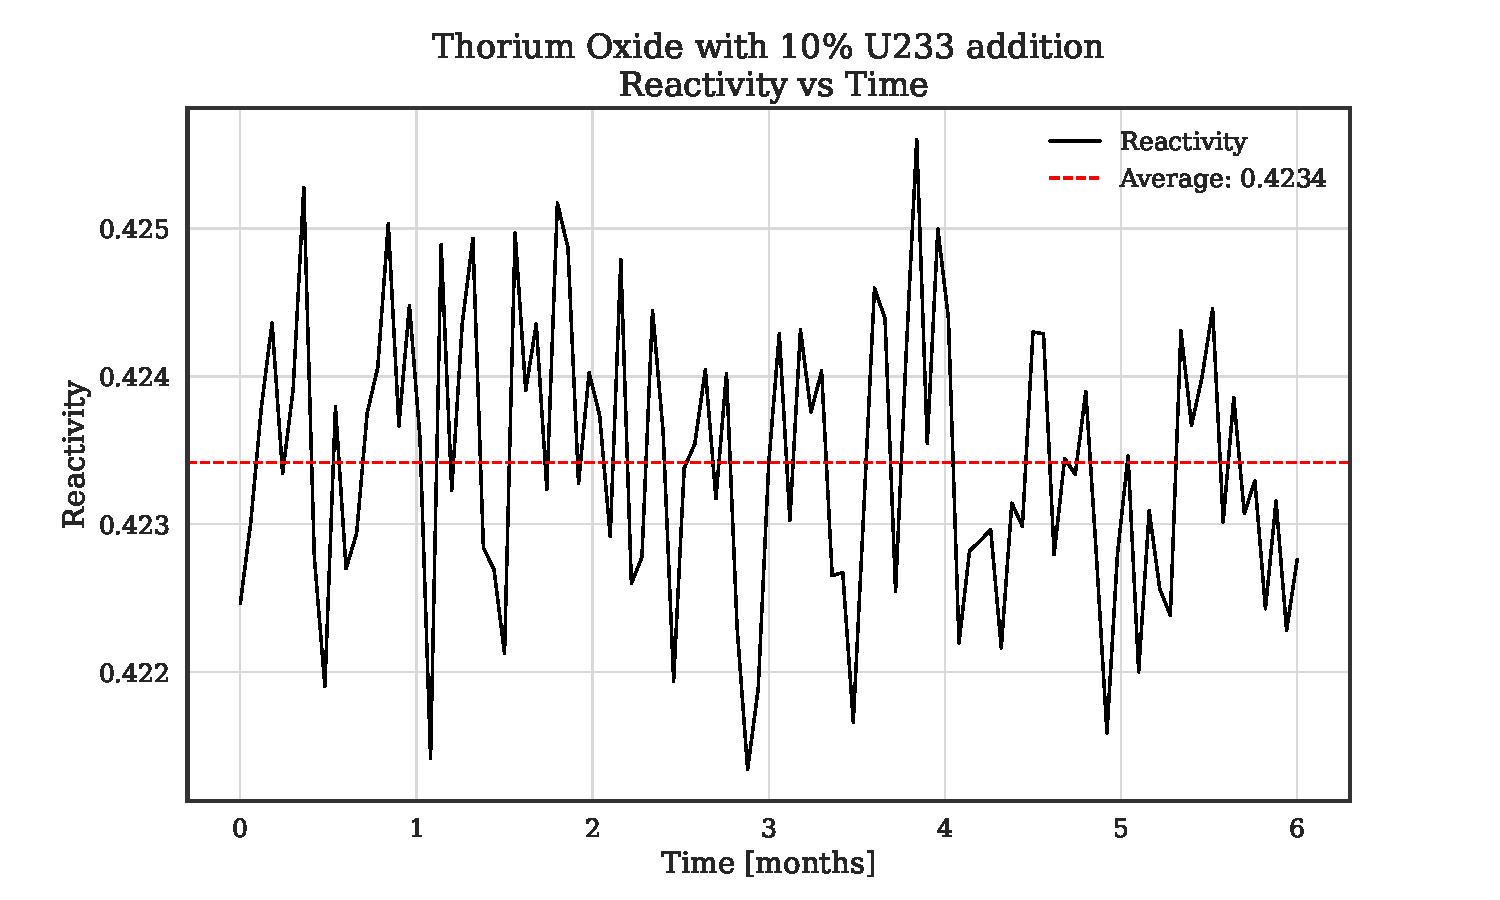
\includegraphics[width=0.75\textwidth, scale=0.75]{Kap7/Figures_Kap7/Reactivity_vs_Time_ThOX_U233_10.pdf}
    \caption{Reactivity of the simulation of a PWR fuel assembly using ThOX at \(10 \, \%\) \(\prescript{233}{}{U}\) concentration.}
    \label{fig:reactivity_th_u233_10}   
\end{figure}

\begin{figure}
    \centering
    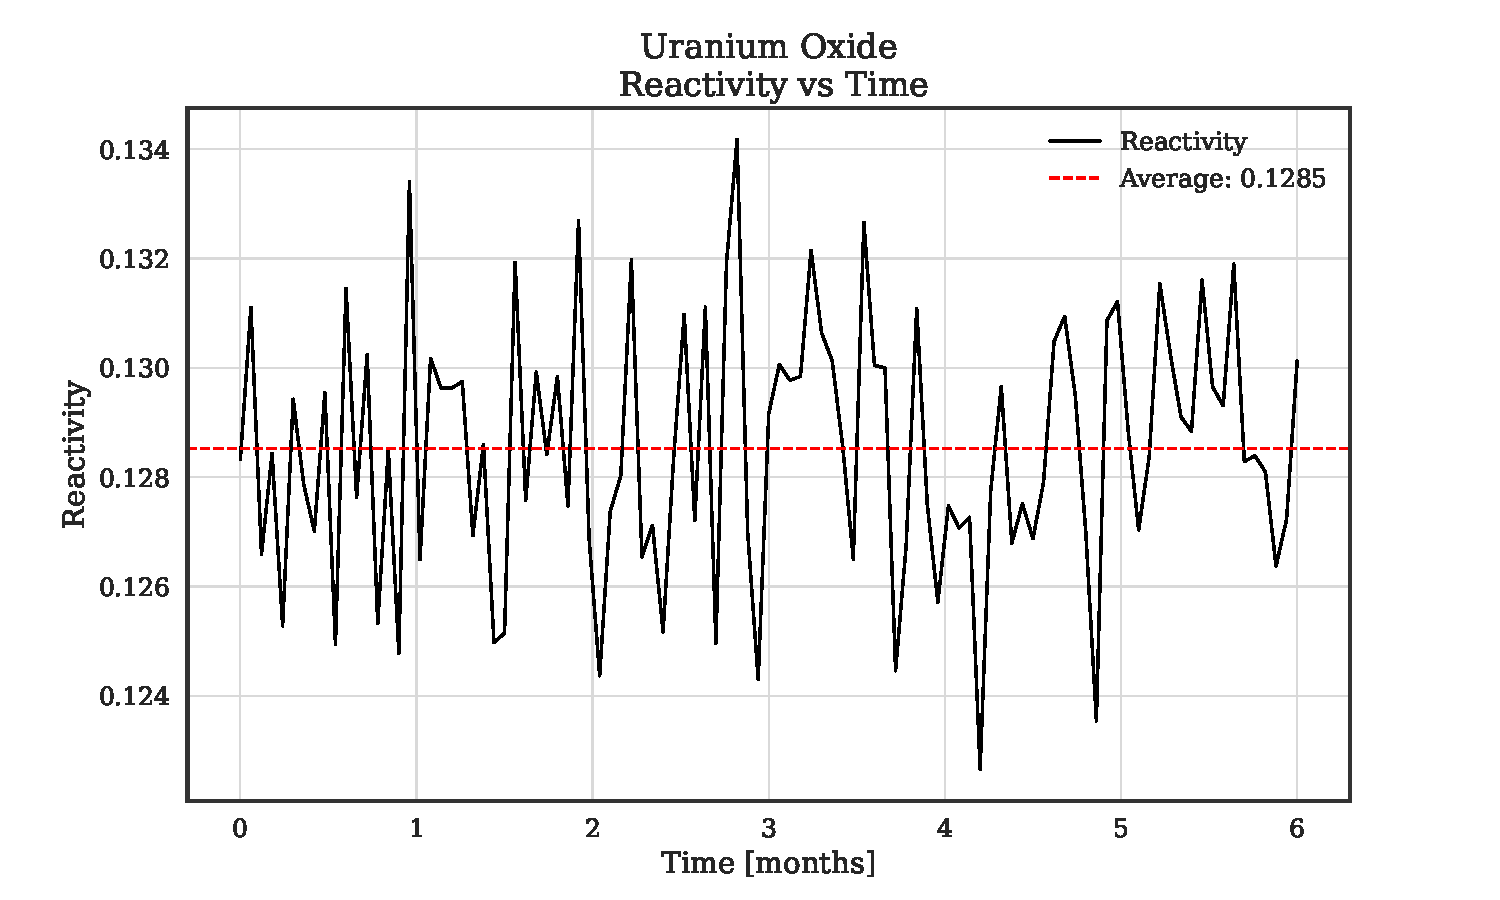
\includegraphics[width=0.75\textwidth, scale=0.75]{Kap7/Figures_Kap7/Reactivity_vs_Time_UOX.pdf}
    \caption{Reactivity of the simulation of a PWR fuel assembly using UOX.}
    \label{fig:reactivity_uox}
\end{figure}